\documentclass[12pt]{amsart}

\addtolength{\hoffset}{-2.25cm}
\addtolength{\textwidth}{4.5cm}
\addtolength{\voffset}{-2.5cm}
\addtolength{\textheight}{5cm}
\setlength{\parskip}{0pt}
\setlength{\parindent}{15pt}
\usepackage{listings}
\usepackage{amsthm}
\usepackage{amsmath}
\usepackage[spanish]{babel}
\usepackage[sort&compress, numbers]{natbib}
\usepackage{amssymb}
\usepackage[utf8]{inputenc}
\usepackage[colorlinks = true, linkcolor = thistle, citecolor = thistle, final]{hyperref}
\usepackage{listings}
\usepackage{ragged2e}
\usepackage{subcaption} 
\usepackage{minted}
\usemintedstyle{borland}
\usepackage{multicol}
\usepackage{listings}
\usepackage{xcolor}
\usepackage{graphicx}
\usepackage[sort&compress, numbers]{natbib}
\usepackage{xcolor}
\usepackage{listings}
\usepackage{ragged2e}
\usepackage{graphicx}
\usepackage[sort&compress, numbers]{natbib}
\usepackage{xcolor}
\usepackage{listings}
\usepackage{ragged2e}
\hypersetup{
    colorlinks=true,
    linkcolor=violet,
    filecolor=violet,     
    urlcolor=violet,
    citecolor=violet,
}
\usepackage{graphicx}
\usepackage[sort&compress, numbers]{natbib}
\usepackage{xcolor}
\usepackage{listings}
\usepackage{ragged2e}

\lstset{style=mystyle}
\usepackage{graphicx}
\usepackage{multicol}
\usepackage{ marvosym }
\newcommand{\ds}{\displaystyle}


\pagestyle{myheadings}

\setlength{\parindent}{0in}
\begin{document}

\pagestyle{empty}



\thispagestyle{empty}

{\scshape Simulación} \hfill {\scshape \Large Tarea 6: Sistema Multiagente} \hfill  {\scshape 24/Mar/2021}
\author{C. María Montemayor Palos}
\maketitle

\hrule
\hrule
\bigskip


\section{Objetivo}
Examinar y analizar el efecto estadístico del valor de $p_v$ (de cero a uno en pasos de 0.1) de un sistema multiagente con aplicación epidemiológica, con una vacunación con probabilidad $p_v$ a los agentes al momento de crearlos de tal forma que desde el inicio se encuentren en el estado R y ya no podrán contagiarse ni propagar la infección, y el porcentaje máximo de infectados durante la simulación y el momento (iteración) en el cual se alcanza ese máximo.\cite{dra}.

\section{Metodología}
Para efectos de la tarea se utiliza el programa R versión 4.0.4 \cite{R} para Windows. Los agentes siguen el modelo SIR, en el cual se pueden encontrar en tres estados diferentes: susceptibles, infectados o recuperados. Se considera como parámetros un cuadro de tamaño \texttt{l}$\times$\texttt{l}. en donde se posicionan $n$ agentes uniformemente al azar y con una probabilidad de $p_i$ en el que el agente puede estar infectado desde el inicio. Suponiendo que la infección produce inmunidad en los recuperados, por lo cual solamente los susceptibles podrán ser infectados. La probabilidad de contagio será proporcional a la distancia euclideana entre dos agentes $d(i, j)$ de la siguiente manera:
\begin{equation} 
p_c = \left \{ \begin{array}{ll}
  0, & \text{ si } d(i, j) \geq r, \\
  \displaystyle\frac{r - d}{r}, & \text{ en otro caso,} \end{array}
  \right.
  \label{ec1}
\end{equation}
  donde $r$ es un umbral.

\section{Código}
Se modifica el código de Schaeffer \cite{codigo}. Se establecen los números de agentes y se vacuna con probabilidad \texttt{pv} al momento de crearlos, así no podrán ser infectados en ninguna de las iteraciones posteriores. Se varía dicha probabilidad \texttt{pvvar} de cero a uno en pasos de 0.1. Se generan diez réplicas del experimento.
\renewcommand{\listingscaption}{Código}
\begin{listing}[H]
  \begin{minted}[linenos,mathescape,texcl]{clojure}
l <- 1.5
n <- 50 #Número de agentes
pi <- 0.05 #Probabilidad de infección
pr <- 0.02
v <- l / 30

pvvar <- seq(0,1,0.1) #Variacion de la probablidad de 0 a 1 
infectadosMax <- c()
for(pv in pvvar) { #Incremento en la probabilidad de vacunados
  for(rep in 1:10) { #Replicas del experimento 
  \end{minted}
  \label{codigo1}
\end{listing}
\clearpage

Se generan los gráficos del porcentaje máximo de infectados durante la simulación y el momento (iteración) en el cual se alcanza ese máximo.
\renewcommand{\listingscaption}{Código}
\begin{listing}[H]
  \begin{minted}[linenos,mathescape,texcl]{clojure}
salida <- paste("vacuna=", pv, ".png", sep="")
    png(salida)
    plot(1:length(epidemia), 100 * epidemia / n, xlab="Tiempo", 
                                                 ylab="Porcentaje de infectados",
         main=paste("Vacunados: ",pv * 100, "%"))
    graphics.off()
    infectadosMax <- c(infectadosMax, max(epidemia)) #Se guardan los infectados 
    maximos por cada replica
 
  \end{minted}
  \label{codigo2}
\end{listing}

Se realiza un \texttt{data.frame} para concatenar la probabilidad de vacuna con sus respectivas réplicas y se obtiene el porcentaje de infectados. Se realiza un diagrama violín para visualizar los resultados y se genera un gif de todos los pasos con la librería \texttt{gifski}.

\renewcommand{\listingscaption}{Código}
\begin{listing}[H]
  \begin{minted}[linenos,mathescape,texcl]{clojure}
datos <- data.frame(Probabilidad_de_vacuna = c(rep("0",10),rep("0.1",10),
                                               rep("0.2",10),rep("0.3",10),
                                               rep("0.4",10),rep("0.5",10),
                                               rep("0.6",10),rep("0.7",10),
                                               rep("0.8",10),rep("0.9",10),
                                               rep("1",10)), 
                    Infectados_maximos = (infectadosMax/n)*100)

library(ggplot2)
tiff("t6-Violin.png", units="in", width=12, height=6.8, 
     res=300, compression = 'lzw')
g <- ggplot(datos, aes(Probabilidad_de_vacuna,Infectados_maximos))
g + geom_violin(alpha = 0.5,draw_quantiles = c(0.25, 0.5, 0.75), 
                trim = FALSE,adjust=1.5,aes(fill= Probabilidad_de_vacuna))
+ geom_jitter() + labs(x= "Probabilidad de vacuna",
                       y = "Porcentaje m\u{E1}ximo de infectados", 
                       fill ="Probabilidad de vacuna" )
graphics.off()

#Generación del GIF
library(gifski)
png_files <- list.files( pattern = "p6_t.*png$", full.names = TRUE)
gifski(png_files, gif_file = "animation.gif", width = 800, height = 600, delay = 1)

  \end{minted}
  \label{codigo3}
\end{listing}

\clearpage
\section{Resultados y discusión}
En la figura \ref{fig1} se observa la primera (ver figura \ref{1a}) y la última iteración (ver figura \ref{1b}) de la simulación en la cual los agentes vacunados se encuentran en el estado R (representados con el triángulo color naranja) y muy pocos agentes en estado S (representados con cuadrado color verde). Debido a la vacunación hay una minoría de agentes infectados (representados con círculo color rojo), por lo tanto la propagación de la infección se mantiene baja. Los gifs generados se encuentran en el repositorio de Montemayor \cite{mtyor}.
\begin{figure}[h!]
\centering
\begin{subfigure}[H]{0.4\linewidth}
\includegraphics[width=\linewidth]{p6_t01.png}
\caption{}
\label{1a}
\end{subfigure}
\begin{subfigure}[H]{0.4\linewidth}
\includegraphics[width=\linewidth]{p6_t50.png}
\caption{}
\label{1b}
\end{subfigure}
\caption{Iteración de infectados.}
\label{fig1}
\end{figure}

Se comparan los diferentes diagramas generados del porcentaje de máximo de infectados y el momento en el cual se alcanza ese máximo. En la figura \ref{fig2} se observa que disminuye ligeramente el porcentaje de infectados con la vacunación del 10\% de los agentes como se muestra en la figura \ref{2b} a comparación de la figura \ref{2a} con el 0\% de agentes vacunados.
\begin{figure}[h!]
\centering
\begin{subfigure}[H]{0.4\linewidth}
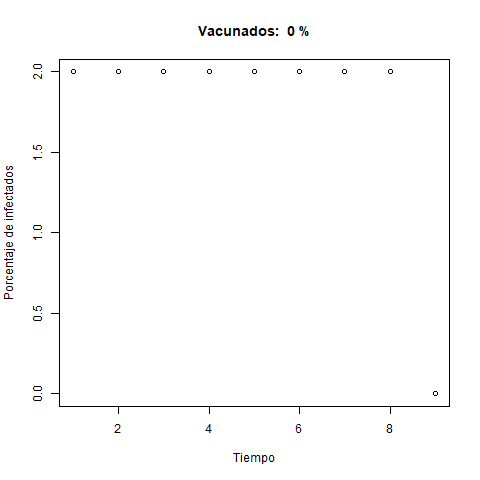
\includegraphics[width=\linewidth]{vacuna=0.png}
\caption{}
\label{2a}
\end{subfigure}
\begin{subfigure}[H]{0.4\linewidth}
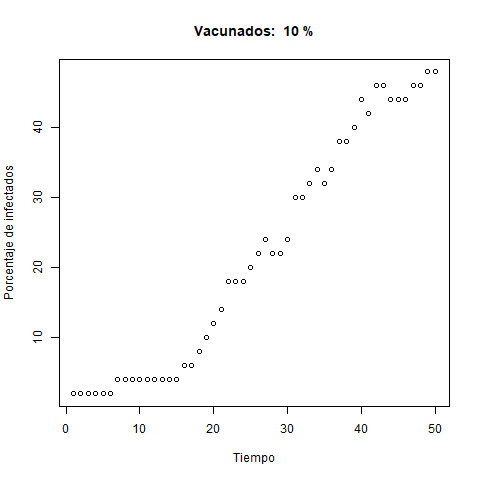
\includegraphics[width=\linewidth]{vacuna=0.1.png}
\caption{}
\label{2b}
\end{subfigure}
\caption{Comparación del porcentaje de máximo de infectados y el momento en el cual se alcanza el máximo.}
\label{fig2}
\end{figure}

\clearpage
En la figura \ref{fig3} se compara el porcentaje de infectados, en la cual se logra apreciar un cambio radical entre la vacunación del 50\% de los agentes (ver figura \ref{3a}) y cuando los agentes están vacunados al 100\% logrando así un porcentaje de infección nulo (ver figura \ref{3b}).
\begin{figure}[h!]
\centering
\begin{subfigure}[H]{0.45\linewidth}
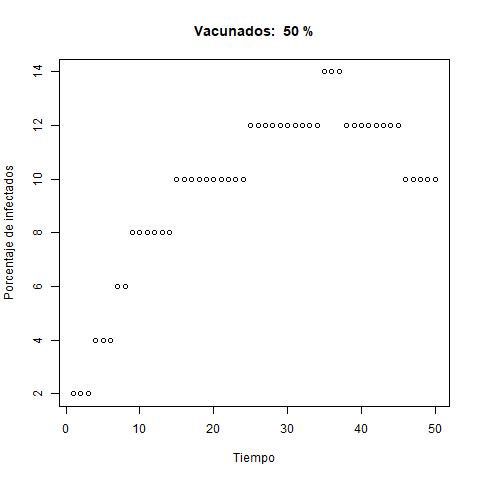
\includegraphics[width=\linewidth]{vacuna=0.5.png}
\caption{}
\label{3a}
\end{subfigure}
\begin{subfigure}[H]{0.45\linewidth}
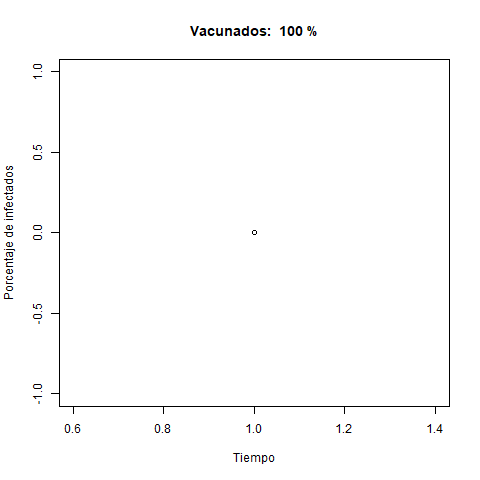
\includegraphics[width=\linewidth]{vacuna=1.png}
\caption{}
\label{3b}
\end{subfigure}
\caption{Comparación del porcentaje de máximo de infectados y el momento en el cual se alcanza el máximo.}
\label{fig3}
\end{figure}

En la figura \ref{fig4} se muestran los gráficos de violín generados variando la probabilidad $p_v$. Como se puede apreciar en dicha figura, cuando se aumenta la probabilidad de vacunación, el porcentaje de infectados disminuye. 
\begin{figure} [h!]
    \centering
    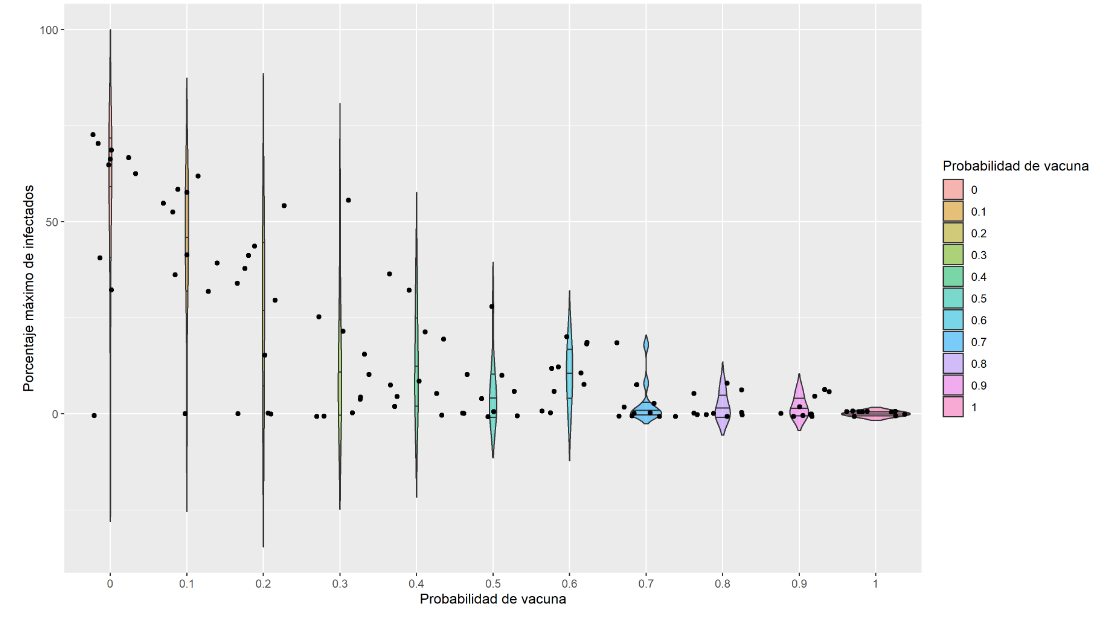
\includegraphics[width=1\textwidth]{t6-violin.png}
    \caption{Gráficas de violín del porcentaje máximo de infectados variando la probabilidad de vacuna.}
    \label{fig4}
\end{figure}

\section{Conclusión}
Como es de esperarse, a mayor probabilidad de vacunación, menor porcentajde de infectados. Al estar los agentes vacunados desde el inicio, se garantiza que disminuyan de manera más rápida los contagios.

\section{Reto 1}
El objetivo del primer reto consiste en cambiar los patrones de movimiento a que no tengan una trayectoria fija los agentes, a que utilice el modelo de punto intermedio aleatorio (inglés: random waypoint model): cada agente tiene una posición meta $(x, y)$ hacia al cual se mueve con una velocidad $v$; al alcanzar (o superar) su meta, elige al azar una nueva meta uniformemente al azar. La velocidad de cada agente es una constante, normalmente distribuido sobre la población de agentes. El objetivo es examinar si surgieron cambios en el efecto de $p_v$ por esta modificación.

Se modificó el código de Schaeffer \cite{codigo} y se apoyó en el repositorio de Llano \cite{llano}. Se realiza un \texttt{data.frame} en el cual se guardan las posiciones metas.
\renewcommand{\listingscaption}{Código}
\begin{listing}[H]
  \begin{minted}[linenos,mathescape,texcl]{clojure}
pvvar <- seq(0,1,0.1) #Variacion de la probablidad de 0 a 1 
infectadosMax <- c()
for(pv in pvvar) { #Incremento en la probabilidad de vacunados
  for(rep in 1:10) { #Replicas del experimento 
    agentes <- data.frame(x = double(), y = double(), 
                          pmx = double(), pmy = double(), 
                          dx = double(), dy = double(),  
                          estado  = character(), rest = integer())
  \end{minted}
  \label{codigo4}
\end{listing}

Se generan los pasos por recorrer y las velocidades de los agentes hasta sus puntos meta.

\renewcommand{\listingscaption}{Código}
\begin{listing}[H]
  \begin{minted}[linenos,mathescape,texcl]{clojure}
      pasos <- sample(5:50,1) #Numero de pasos por recorrer
      xc <- runif(1,0,l) #Punto inicial en x
      yc <- runif(1,0,l) #Punto inicial en y
      px = runif(1,0,l) #Punto meta en x
      py = runif(1,0,l) #Punto meta en y
      
      vx = ((px - xc)/pasos) #Velocidad a la meta en X
      vy = ((py - yc)/pasos) #Velocidad a la meta en Y
      agentes <- rbind(agentes, data.frame(x = xc, y = yc, pmx = px, pmy = py,
                                           dx = vx, dy = vy,
                                           estado = e,rest = pasos))
  \end{minted}
  \label{codigo5}
\end{listing}
\clearpage
Se generan los nuevos puntos meta y sus velocidades.
\renewcommand{\listingscaption}{Código}
\begin{listing}[H]
  \begin{minted}[linenos,mathescape,texcl]{clojure}
    } else {
          pasos <- sample(5:30,1)
          a$rest <- pasos
          a$x <- a$pmx
          a$y <- a$pmy
          a$pmx <- runif(1,0,l)
          a$pmy <- runif(1,0,l)
          vx = (a$pmx - a$x)/pasos
          vy = (a$pmy - a$y)/pasos
          a$dx <- vx
          a$dy <- vy
  \end{minted}
  \label{codigo5}
\end{listing}

En conlusión comparando los resultados de los diagramas violín generados, podemos observar en la figura \ref{fig5} que existe un comportamiento similar al de la figura \ref{fig4}, pero los porcentajes de contagio son ligeramente mayores debido a que este tipo de movimiento de los agentes provoca que tengan mayor contacto con los demás. 
\begin{figure} [h!]
    \centering
    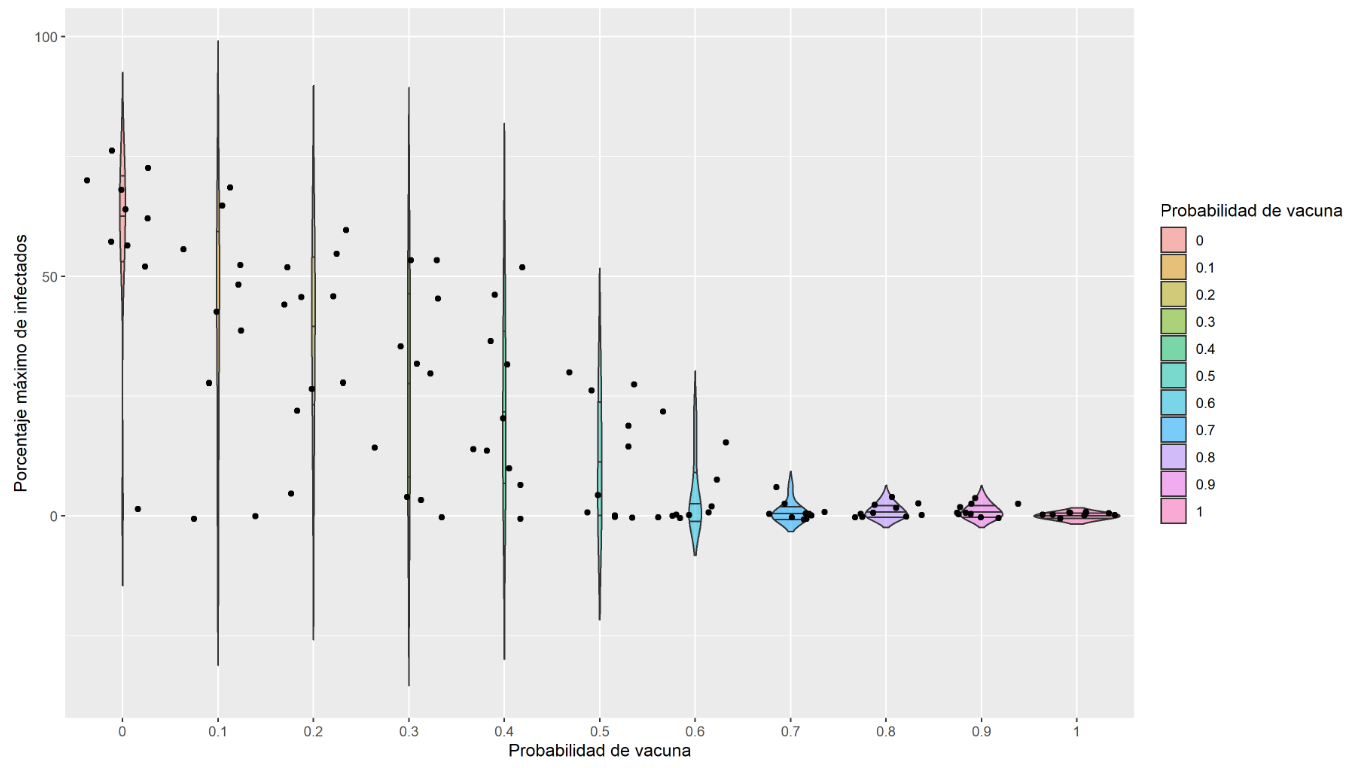
\includegraphics[width=1\textwidth]{t6r1.png}
    \caption{Gráficas de violín del porcentaje máximo de infectados variando la probabilidad de vacuna.}
    \label{fig5}
\end{figure}
\clearpage
\section{Reto 2}
El reto dos consiste en que los agentes tienen amistades: si se encuentran una distancia euclideana no mayor a $r_a$ de un amigo suyo, se disminuyen su velocidad a la mitad por $k_a$ iteraciones (para saludar a su amigo). Cada par de agentes tiene una amistad con una probabilidad $p_a$. Examina nuevamente si surgieron cambios en el efecto de $p_v$ por esta modificación, con valores $0 < r_a < 1$, $k_a > 1$ y $0 < p_a \ll 1$.
Se asignan los valores a elección para \texttt{ra}, \texttt{pa}, y \texttt{ka}.
\renewcommand{\listingscaption}{Código}
\begin{listing}[H]
  \begin{minted}[linenos,mathescape,texcl]{clojure}
    r <- 0.1
    ra <- 0.7
    pa <- 0.4
    ka <- 8
    tmax <- 50
    digitos <- floor(log(tmax, 10)) + 1
    for (tiempo in 1:tmax) {
  \end{minted}
  \label{codigo5}
\end{listing}

Se modifica el código para que los agentes disminuyan su velocidad cada que se encuentren a un amigo suyo.

\renewcommand{\listingscaption}{Código}
\begin{listing}[H]
  \begin{minted}[linenos,mathescape,texcl]{clojure}
if (d < ra) { # umbral amistad
     p <- (r - d) / r
    if (runif(1) < pa) {
        for (i in 1:ka) { # iteraciones por la mitad
            dx <- (a1$x - a2$x)/2
            dy <- (a1$y - a2$y)/2
  \end{minted}
  \label{codigo5}
\end{listing}

En conclusión se puede observar en la figura \ref{fig6} que es similar a las figuras \ref{fig5} y \ref{fig4} debido a que al inicio se vacunan los agentes, por lo tanto no hay un índice elevado de infectados, pero existe cierta diferencia en la que disminuye de manera más rápida el porcentaje de infectados a pesar de que los agentes disminuyen sus velocidades cuando se encuentran con un amigo.
\begin{figure} [h!]
    \centering
    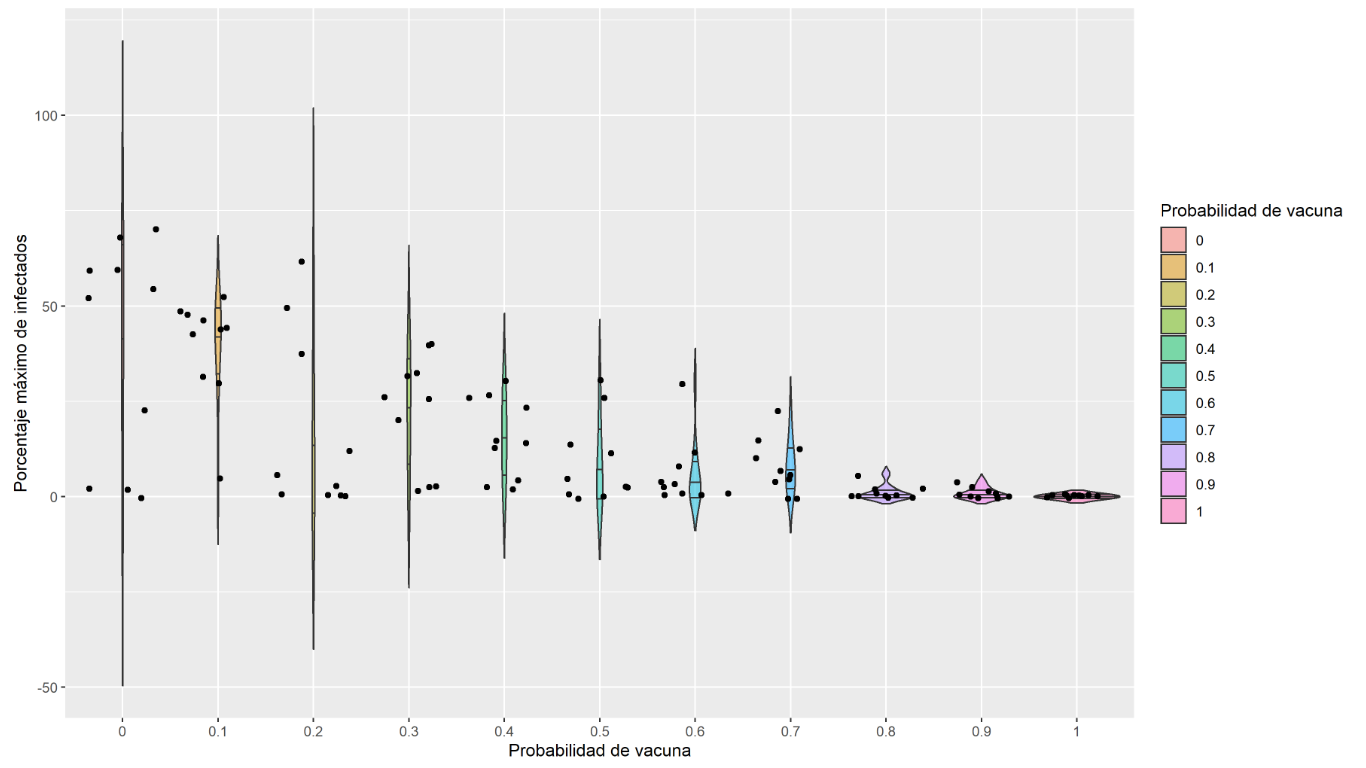
\includegraphics[width=0.85\textwidth]{t6r2.png}
    \caption{Gráficas de violín del porcentaje máximo de infectados variando la probabilidad de vacuna.}
    \label{fig6}
\end{figure}

\clearpage
\bibliography{referencias}
\bibliographystyle{plainnat}


\end{document}

